% PASC talk sub-section: Matrix-Free High-Order CVFEM at Scale
% Standalone, compilable Beamer source. No external image files: all figures
% are inline pgfplots/tikz so it builds anywhere with a TeX + pgfplots install.
%
% Style is built to approximate the existing MARS PASC deck (internal-notes/mars.pdf,
% a PowerPoint export -- no .tex source exists in the repo to reuse). We mirror:
%   - white background, large plain BLACK SANS-SERIF title (PowerPoint default,
%     no boxes / no colored title bar)
%   - bold dark section sub-header line ("Throughput on GH200" style)
%   - flat bullets with "o" style sub-bullets
%   - blue/orange plot palette + light grey grid (matches the deck's charts)
%   - bottom institutional logo strip: UniDistance.ch, USI/Euler, HSLU Luzern,
%     CSCS, PASC -- the same five marks at the foot of every mars.pdf slide
%
% Drop-in: if a shared mars-beamer-theme.sty is later created, replace the
% PREAMBLE block below with \input{mars-beamer-theme}.
\documentclass[aspectratio=43,11pt]{beamer}

% ---------------------------------------------------------------------------
% PREAMBLE (theme approximation of internal-notes/mars.pdf)
% ---------------------------------------------------------------------------
\usepackage[T1]{fontenc}
\usepackage[utf8]{inputenc}
% The deck is a PowerPoint export: plain black sans-serif titles + body
% (Arial-like). Helvetica as the default family is the closest free match.
\usepackage{helvet}
\renewcommand{\familydefault}{\sfdefault}
\usepackage{sansmath}           % sans-serif math so formulas match body font
\usepackage{amsmath}
\usepackage{tikz}
\usepackage{pgfplots}
\pgfplotsset{compat=1.16}
\usepgfplotslibrary{groupplots}
\usetikzlibrary{positioning}

% Strip all the beamer chrome: no navigation, no shadows, no rounded blocks.
\usetheme{default}
\useinnertheme{default}
\useoutertheme{default}
\setbeamertemplate{navigation symbols}{}
\setbeamercolor{background canvas}{bg=white}

% Deck color accents (sampled from mars.pdf charts/headers).
\definecolor{marsblue}{HTML}{2C7FB8}   % primary plot line / accent
\definecolor{marsorange}{HTML}{F07E26}  % secondary plot line
\definecolor{marsdark}{HTML}{222222}    % title / body text
\definecolor{marsgrey}{HTML}{555555}    % sub-header
\definecolor{marsgreen}{HTML}{2E8B57}   % third accent (convergence p4)
\definecolor{marsgridgrey}{HTML}{CCCCCC}

\setbeamercolor{frametitle}{fg=marsdark}
\setbeamercolor{normal text}{fg=marsdark}
\setbeamercolor{structure}{fg=marsblue}
\setbeamercolor{itemize item}{fg=marsdark}
\setbeamercolor{itemize subitem}{fg=marsgrey}

% Big plain SANS-SERIF title, no background bar -- matches the deck's
% free-floating PowerPoint titles (large, plain black, not boxed).
\setbeamerfont{frametitle}{size=\Large,series=\mdseries,family=\sffamily}
\setbeamertemplate{frametitle}{%
  \vspace{0.35em}\hspace{0.2em}\insertframetitle\par
  \vspace{-0.2em}{\color{marsgridgrey}\rule{\linewidth}{0.4pt}}}

% Flat bullets: round dark dot, "o" sub-bullet (PowerPoint o-style in the deck).
\setbeamertemplate{itemize item}{\small\raise0.15ex\hbox{\textbullet}}
\setbeamertemplate{itemize subitem}{\footnotesize\raise0.1ex\hbox{$\circ$}}
\setbeamertemplate{itemize subsubitem}{\scriptsize--}
\setbeamerfont{itemize/enumerate body}{size=\footnotesize}
\setbeamerfont{itemize/enumerate subbody}{size=\footnotesize}

% Bold dark sub-header command (the "Throughput on GH200" style line).
\newcommand{\subhead}[1]{{\color{marsdark}\bfseries #1}\par\vspace{0.2em}}

% ---------------------------------------------------------------------------
% Institutional logo strip (text/tikz placeholders for USI, CSCS, PASC, HSLU,
% UniDistance -- the same five marks that sit at the bottom of mars.pdf). Kept
% as styled text so the file compiles with no external logo assets.
% ---------------------------------------------------------------------------
\newcommand{\logostrip}{%
  \begin{tikzpicture}[remember picture,overlay]
    \node[anchor=south,inner sep=0pt] at ([yshift=4pt]current page.south) {%
      \tiny\color{marsgrey}%
      \begin{tabular}{ccccc}
        \textbf{UniDistance.ch} & \textbf{USI} Euler Inst. &
        \textbf{HSLU} Luzern & \textcolor{marsorange}{\textbf{CSCS}} &
        \textcolor{marsblue}{\textbf{PASC}}\\
      \end{tabular}};
  \end{tikzpicture}}

% ---------------------------------------------------------------------------
% Shared pgfplots style so every chart matches the deck (light grid, no box).
% ---------------------------------------------------------------------------
\pgfplotsset{
  marsplot/.style={
    width=\linewidth, height=0.52\linewidth,
    tick align=outside, tick pos=left,
    axis line style={marsgrey},
    label style={font=\scriptsize,color=marsdark},
    tick label style={font=\tiny,color=marsdark},
    title style={font=\footnotesize\bfseries,color=marsdark},
    legend style={font=\tiny,draw=none,fill=none,legend cell align=left},
    grid=both,
    major grid style={marsgridgrey,line width=0.3pt},
    minor grid style={marsgridgrey!50,line width=0.2pt},
  },
  marsline/.style={mark=*,mark size=1.2pt,line width=1.2pt},
}

% Make inline math render in the sans family too, so $p$, exponents, etc.
% match the Helvetica body instead of falling back to Computer Modern serif.
\sansmath

\begin{document}

% ===========================================================================
% Section divider (this is a SUB-SECTION of the pump-FSI talk).
% ===========================================================================
\section{Matrix-Free High-Order CVFEM at Scale}

% ===========================================================================
% FRAME 1 -- the assembly wall
% ===========================================================================
\begin{frame}{Matrix-free high-order CVFEM: past the assembly wall}
  \begin{columns}[T]
    \begin{column}{0.50\textwidth}
      \subhead{The assembled wall}
      \begin{itemize}
        \item Assembled CVFEM storage explodes with order $p$:\\
              $\text{nnz/row}\sim(2p{+}1)^3$
        \item Bytes/DOF grow $324\!\to\!40{,}500$ from $p{=}1$ to $p{=}7$
        \item Assembly infeasible beyond $p\!\approx\!2\text{--}3$
      \end{itemize}
      \vspace{0.4em}
      \subhead{Matrix-free answer}
      \begin{itemize}
        \item High-order matrix-free CVFEM
              (Knaus / Nalu-Wind scheme), GPU-native in MARS
        \item \textbf{Trilinos-free}: cstone octree + own CSR + cuSPARSE + Hypre
        \item Store per-element geometry \emph{once}; recompute the
              $O(p^4)$ sum-factorized apply each matvec
      \end{itemize}
    \end{column}
    \begin{column}{0.50\textwidth}
      \begin{figure}
      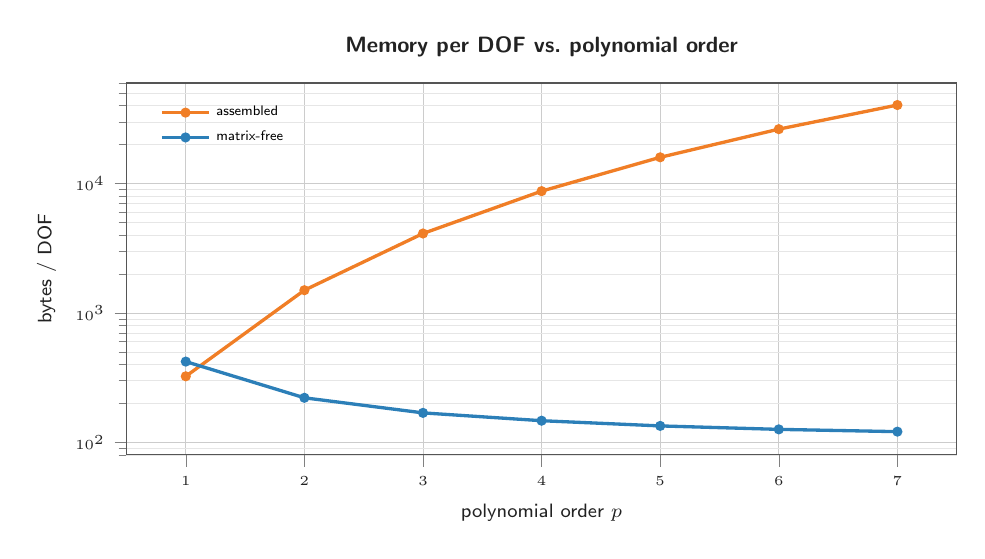
\begin{tikzpicture}
        \begin{semilogyaxis}[marsplot,
            title={Memory per DOF vs.\ polynomial order},
            xlabel={polynomial order $p$}, ylabel={bytes / DOF},
            xmin=0.5,xmax=7.5, xtick={1,2,3,4,5,6,7},
            ymin=80,ymax=60000,
            legend pos=north west]
          % assembled: storage blows up as (2p+1)^3
          \addplot[marsline,color=marsorange] coordinates {
            (1,324)(2,1500)(3,4116)(4,8748)(5,15972)(6,26364)(7,40500)};
          \addlegendentry{assembled}
          % matrix-free: geometry-only footprint, decreasing per-DOF
          \addplot[marsline,color=marsblue] coordinates {
            (1,421)(2,221)(3,169)(4,147)(5,134)(6,126)(7,121)};
          \addlegendentry{matrix-free}
        \end{semilogyaxis}
      \end{tikzpicture}
      \end{figure}
      \footnotesize\color{marsgrey}
      Crossover at $p{=}1$; for $p\!\ge\!2$ matrix-free is the only
      affordable option.
    \end{column}
  \end{columns}
  \logostrip
  \note{Set up the core problem: assembled high-order CVFEM is a dead end on
    memory (nnz/row ~ (2p+1)^3). Matrix-free trades storage for FLOPs --
    recompute the sum-factorized operator apply. Emphasize this is the
    established Knaus/Nalu-Wind scheme, but our reimplementation is GPU-native
    and Trilinos-free (cstone + own CSR + cuSPARSE + Hypre). The plot is the
    hook: the assembled curve is the wall.}
\end{frame}

% ===========================================================================
% FRAME 2 -- the key slide: performance + memory vs assembled
% ===========================================================================
\begin{frame}{Performance \& memory vs.\ the assembled kernel}
  \subhead{Single-GPU H100 order sweep}
  \begin{columns}[T]
    \begin{column}{0.46\textwidth}
      \begin{itemize}
        \item Throughput \textbf{flat with order}: 4.3--8.0 GDOF/s
              ($p{=}7\!\approx\!p{=}1$)
        \item Memory \emph{drops} $421\!\to\!121$ B/DOF; assembled up to
              \textbf{336$\times$} larger at $p{=}7$
        \item $p{=}1$: assembled SpMV wins one matvec (9.2 vs 6.0 GDOF/s);
              $p\!\ge\!2$ matrix-free is the \emph{only} option, no penalty
        \item Kernel: \textbf{75\%} occupancy, $\sim$2 TB/s ($\approx$60\% peak),
              L1-bound; FP64 tensor cores measured -- \emph{don't} help
      \end{itemize}
    \end{column}
    \begin{column}{0.52\textwidth}
      \begin{figure}
      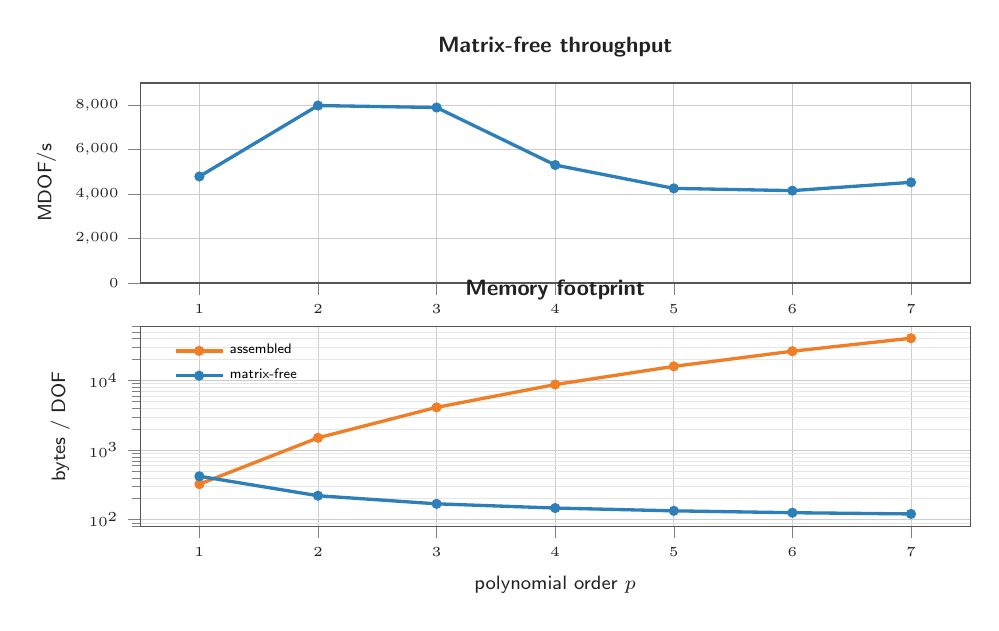
\begin{tikzpicture}
        \begin{groupplot}[group style={group size=1 by 2,
              vertical sep=0.55cm}, marsplot, height=0.34\linewidth,
              xmin=0.5,xmax=7.5, xtick={1,2,3,4,5,6,7}]
          % top: throughput vs p (the "flat" story)
          \nextgroupplot[title={Matrix-free throughput},
              ylabel={MDOF/s}, ymin=0, ymax=9000]
            \addplot[marsline,color=marsblue] coordinates {
              (1,4794)(2,7984)(3,7895)(4,5309)(5,4258)(6,4157)(7,4530)};
          % bottom: memory vs p (the "drops" story, log axis)
          \nextgroupplot[title={Memory footprint},
              xlabel={polynomial order $p$}, ylabel={bytes / DOF},
              ymode=log, ymin=80, ymax=60000, legend pos=north west]
            \addplot[marsline,color=marsorange] coordinates {
              (1,324)(2,1500)(3,4116)(4,8748)(5,15972)(6,26364)(7,40500)};
            \addlegendentry{assembled}
            \addplot[marsline,color=marsblue] coordinates {
              (1,421)(2,221)(3,169)(4,147)(5,134)(6,126)(7,121)};
            \addlegendentry{matrix-free}
        \end{groupplot}
      \end{tikzpicture}
      \end{figure}
    \end{column}
  \end{columns}
  \logostrip
  \note{This is the money slide. Two messages: (1) throughput is essentially
    flat in p -- high order is "free" on time; (2) memory goes the right way
    for matrix-free and the wrong way for assembled (up to 336x at p=7). Be
    honest about the low-order caveat: at p=1 the assembled tensor kernel wins
    a single matvec (9.2 vs 6.0 GDOF/s), which is the textbook result. The
    crossover is real and at p>=2 matrix-free wins on both axes. The
    occupancy/bandwidth and FP64-tensor-core points pre-empt the "why not
    tensor cores" question -- we measured it, it does not help.}
\end{frame}

% ===========================================================================
% FRAME 3 -- accuracy & validation
% ===========================================================================
\begin{frame}{Accuracy \& validation}
  \begin{columns}[T]
    \begin{column}{0.48\textwidth}
      \subhead{High order pays off}
      \begin{itemize}
        \item Convergence reproduces the reference (paper Table 1):
              $\sim p{+}1$ order
        \item At a fixed $\sim$2{,}200 DOFs, $p{=}4$ is
              \textbf{$\sim$570$\times$} more accurate than $p{=}1$
      \end{itemize}
      \vspace{0.4em}
      \subhead{Validation}
      \begin{itemize}
        \item GPU apply \textbf{bit-exact} vs an independent host reference,
              $p{=}1..7$ (machine precision)
        \item Consistent: annihilates linears on sheared / distorted meshes
        \item Verified faithful to the Knaus paper's Algorithm 2
      \end{itemize}
    \end{column}
    \begin{column}{0.52\textwidth}
      \begin{figure}
      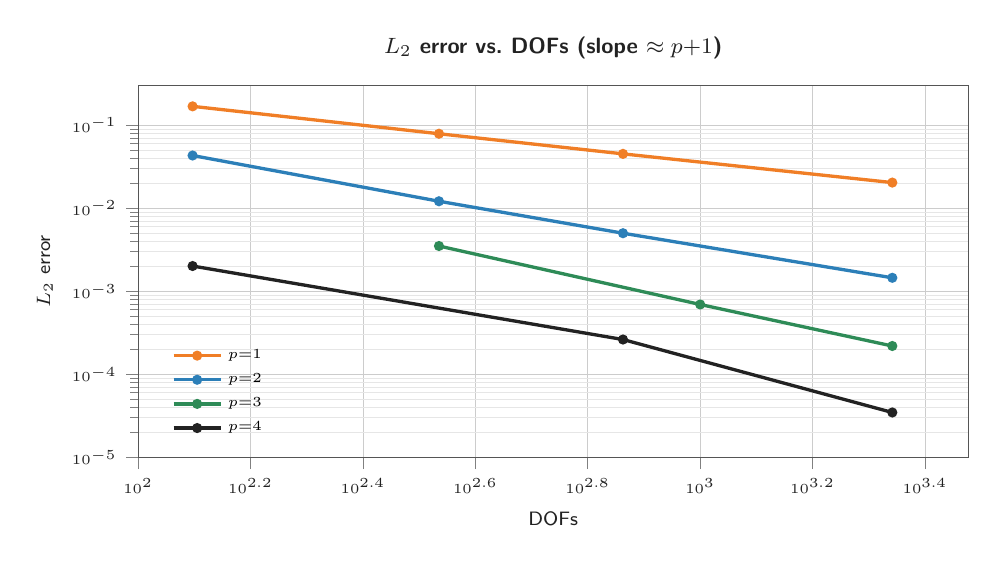
\begin{tikzpicture}
        \begin{loglogaxis}[marsplot,
            title={$L_2$ error vs.\ DOFs (slope $\approx p{+}1$)},
            xlabel={DOFs}, ylabel={$L_2$ error},
            xmin=100,xmax=3000, ymin=1e-5,ymax=3e-1,
            legend pos=south west]
          \addplot[marsline,color=marsorange] coordinates {
            (125,1.68e-1)(343,7.86e-2)(729,4.50e-2)(2197,2.03e-2)};
          \addlegendentry{$p{=}1$}
          \addplot[marsline,color=marsblue] coordinates {
            (125,4.30e-2)(343,1.21e-2)(729,4.99e-3)(2197,1.45e-3)};
          \addlegendentry{$p{=}2$}
          \addplot[marsline,color=marsgreen] coordinates {
            (343,3.50e-3)(1000,6.92e-4)(2197,2.19e-4)};
          \addlegendentry{$p{=}3$}
          \addplot[marsline,color=marsdark] coordinates {
            (125,2.01e-3)(729,2.62e-4)(2197,3.47e-5)};
          \addlegendentry{$p{=}4$}
        \end{loglogaxis}
      \end{tikzpicture}
      \end{figure}
      \footnotesize\color{marsgrey}
      Steepening slopes confirm $p{+}1$ convergence; the vertical gap at fixed
      DOFs is the high-order payoff.
    \end{column}
  \end{columns}
  \logostrip
  \note{Two claims to land: correctness and the value of high order. The
    loglog plot shows steepening slopes (p+1) -- standard high-order signature.
    The killer comparison is vertical at fixed ~2200 DOFs: p=4 is ~570x more
    accurate than p=1 for the same unknowns. Validation: bit-exact GPU-vs-host
    for p=1..7, consistency (kills linears) on distorted meshes, and we checked
    we match Algorithm 2 of the Knaus paper. This buys credibility before the
    scaling claims.}
\end{frame}

% ===========================================================================
% FRAME 4 -- scaling & outlook
% ===========================================================================
\begin{frame}{Scaling \& outlook}
  \begin{columns}[T]
    \begin{column}{0.48\textwidth}
      \subhead{Toward trillions of DOFs}
      \begin{itemize}
        \item Weak scaling on block hex meshes block\_2M $\to$ block\_64M
              on GH200 \textcolor{marsorange}{\textbf{(runs in progress)}}
        \item Procedural per-rank mesh generation -- no mesh file, validated
              identical to the block meshes
        \item Path to $10^{9}$--$10^{12}$ DOF
              ($\sim$3000 GH200 at the current per-GPU footprint)
      \end{itemize}
      \vspace{0.3em}
      \subhead{Differentiator}
      \begin{itemize}
        \item Native \textbf{unstructured AMR} on the cstone octree --
              Nalu-Wind / Kynema-UGF use structured-AMR overset
      \end{itemize}
    \end{column}
    \begin{column}{0.52\textwidth}
      \begin{figure}
      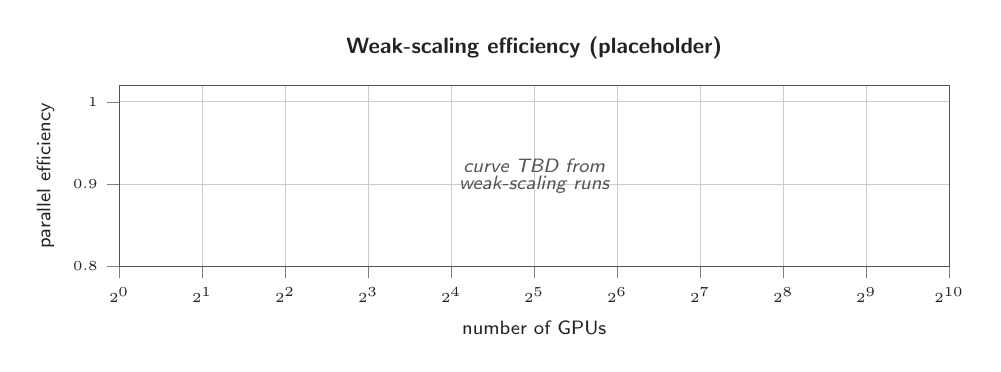
\begin{tikzpicture}
        % PLACEHOLDER: parallel-efficiency axis. Curve to be filled from the
        % multi-rank weak-scaling runs now in progress (block_2M..block_64M).
        \begin{axis}[marsplot, height=0.32\linewidth,
            title={Weak-scaling efficiency \textit{(placeholder)}},
            xlabel={number of GPUs}, ylabel={parallel efficiency},
            xmode=log, log basis x=2,
            xmin=1,xmax=1024, ymin=0.8,ymax=1.02,
            ytick={0.8,0.9,1.0}]
          % intentionally empty -- TODO: addplot weak-scaling data here
          \node[font=\scriptsize\itshape,color=marsgrey,align=center]
            at (axis cs:32,0.91) {curve TBD from\\[-2pt]weak-scaling runs};
        \end{axis}
      \end{tikzpicture}
      \vspace{0.4em}
      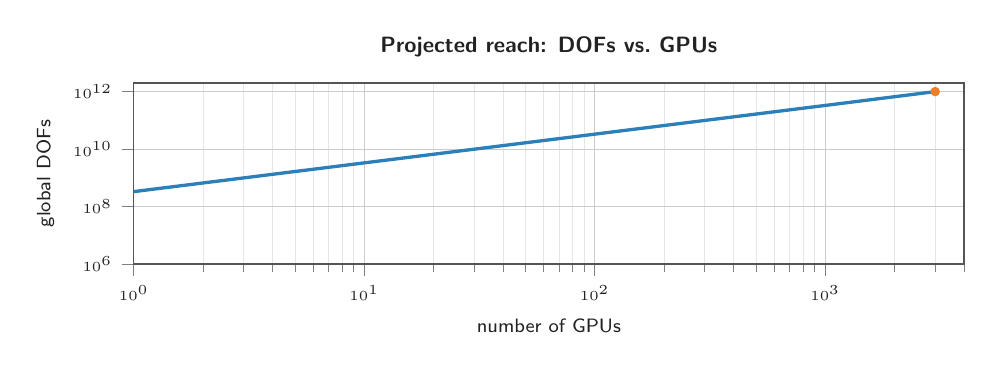
\begin{tikzpicture}
        % small projection: global DOFs vs #GPUs out to 1e12
        \begin{loglogaxis}[marsplot, height=0.32\linewidth,
            title={Projected reach: DOFs vs.\ GPUs},
            xlabel={number of GPUs}, ylabel={global DOFs},
            xmin=1,xmax=4000, ymin=1e6,ymax=2e12,
            log basis x=10]
          % ~3.3e8 DOF/GPU at the current footprint -> 1e12 at ~3000 GPUs
          \addplot[marsline,color=marsblue,mark=none] coordinates {
            (1,3.3e8)(10,3.3e9)(100,3.3e10)(1000,3.3e11)(3000,1e12)};
          \addplot[only marks,mark=*,mark size=1.5pt,color=marsorange]
            coordinates {(3000,1e12)};
          \node[font=\scriptsize,color=marsorange,anchor=south east]
            at (axis cs:3000,1e12) {$10^{12}$};
        \end{loglogaxis}
      \end{tikzpicture}
      \end{figure}
    \end{column}
  \end{columns}
  \logostrip
  \note{Close on scale and what sets MARS apart. The efficiency plot is a
    DELIBERATE PLACEHOLDER -- say "weak-scaling runs are in progress" and that
    the curve will be dropped in from block_2M..block_64M on GH200. The
    projection line is the trillion-DOF narrative: at the current per-GPU
    footprint, ~3000 GH200 reach 1e12 DOF, enabled by procedural per-rank mesh
    gen (no mesh file, validated identical to the block meshes). Final
    differentiator: native unstructured AMR on the cstone octree, vs the
    structured-AMR overset approach in Nalu-Wind / Kynema-UGF.}
\end{frame}

\end{document}
